%% Media firma del representante legal en el pie de página,
%% siguiendo el formato usado por el Subdocumento 9.
% Tamaño físico del cuerpo en el PDF (un bp equivale a un punto PDF).
\makeatletter
\renewcommand{\@xipt}{11.1}
\makeatother
\AtBeginDocument{\normalsize}

% pdflscape gira la página al visualizarla. El pie se compone en sus
% coordenadas de lectura, en la esquina superior derecha de la hoja sin girar.
\AddToHook{env/landscape/before}{\clearpage}
\AddToHook{env/landscape/begin}{%
  \fancyfoot[R]{\begin{tikzpicture}[remember picture,overlay]
    \node[rotate=90,anchor=south east,inner sep=0pt,align=right]
      at ([xshift=-13mm,yshift=-16mm]current page.north east)
      {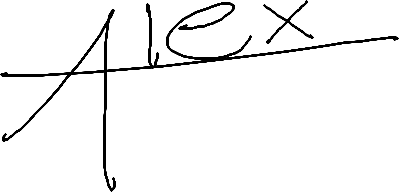
\includegraphics[height=6mm]{logo/FIRMA_Alex_Aravena_transparente.png}\\[-2pt]
       {\LFXchico Media firma: \LFXrepresentante}\\[-2pt]
       {\intermedium\fontsize{9pt}{11pt}\selectfont\LFXfoliotexto}};
  \end{tikzpicture}}}
\renewcommand{\LFXpiederecho}{%
  \begingroup\LFXpiebase
  \begin{tabular}[b]{@{}r@{}}
    {\color{lafroxGris}\rule{3.4cm}{0.4pt}%
     \begin{tikzpicture}[remember picture,overlay]
       \node[anchor=south east,inner sep=0pt] at (0,1mm)
         {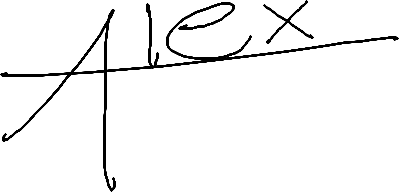
\includegraphics[height=7mm]{logo/FIRMA_Alex_Aravena_transparente.png}};
     \end{tikzpicture}}\\[-1pt]
    {\LFXchico Media firma: \LFXrepresentante}\\
    {\intermedium\fontsize{9pt}{11pt}\selectfont\color{lafroxTinta}\LFXfoliotexto}
  \end{tabular}%
  \endgroup}
